%\documentclass[a4paper,11pt]{article}
\documentclass{article}
%%%%%%%%%%%%%%%%%%%%%%%%%%%%%%%%%%%%%%%%%%%%%%%%%%%%%%%%%%%%%%%%%%%%%%%%%%%%%%%%%%%%%%%%%%%%%%%%%%%%%%%%%%%%%%%%%%%%%%%%%%%%
\usepackage{graphics,graphicx}
\usepackage{amsmath,amssymb,graphics,graphicx}
\usepackage[ansinew]{inputenc}
\usepackage[usenames,dvipsnames]{color}

\graphicspath{{Images/}}
\usepackage{natbib}

\bibpunct{(}{)}{;}{a}{,}{,}

\textheight 24cm \textwidth 17cm \topmargin-2cm
%% \evensidemargin   -0.25cm
\oddsidemargin-0.2cm
%\pagestyle{empty}
\renewcommand{\baselinestretch}{1}

\begin{document}

\title{Pr\'actica 1: FIFA Players Classification}

\author{{Daniel Carmona Pedrajas}}

\date{}
\maketitle

%\title{}

%\address{}

	\section{Arquitectura 1: Feed Forward Neural Network}
		La primera arquitectura que usaremos es tan simple como:
		\begin{enumerate}
			\item Capa densa con 512 neuronas.
		\end{enumerate}
		\subsection{Experimento 1: Configuraci\'on base arbitraria}
		\label{s-a1-e1}
			Usamos la siguiente configuraci\'on:
			\begin{table}[!h]
				\begin{center}
					\begin{tabular}{| c | c | c | c | c | c | c |}
						\textbf{Epochs} & \textbf{Learning rate} & \textbf{Batch size} & \textbf{Activation} & \textbf{Loss} & \textbf{Optimizer} & \textbf{Regularization} \\ \hline
						100 & 0.1 & 512 & ReLU & Categorical Crossentropy & SGD & None
					\end{tabular}
					\caption{Hiperpar\'ametros para el Experimento 1 de la Arquitectura 1}
					\label{tab:hip-a1-e1}
				\end{center}
			\end{table}
		
			Y entrenamos 5 veces para obtener los siguientes resultados:
			\begin{table}[!h]
				\begin{center}
					\begin{tabular}{ c | c | c | c | c | c |}
						\ & \textbf{Train accuracy (\%)} & \textbf{Validation accuracy (\%)} & \textbf{Bias (\%)} & \textbf{Variance (\%)} & \textbf{Training time (s)} \\ \hline
						\textbf{Mean} & 79.38 & 77.94 & 15.61 & 1.44 & 14\\ \hline
						\textbf{Std} & 0.05 & 0.14 & 0.05 & 0.19 & 0 \\ \hline
					\end{tabular}
					\caption{Resultados del Experimento 1 de la Arquitectura 1}
					\label{tab:res-a1-e1}
				\end{center}
			\end{table}
		
			Tener un \textit{bias} alto y una \textit{variance} baja significa que hay margen de mejora antes de llegar al \textit{overfitting} y hay varias posibilidades para conseguir una mejor \textit{accuracy}: a\~nadir m\'as neuronas, entrenar con m\'as \textit{epochs}, ...
		
		\subsection{Experimento 2: Aumentamos \textit{epochs}}
		\label{s-a1-e2}
			Tras el experimento anterior, nos decantamos por entrenar el modelo durante m\'as \textit{epochs} para reducir el \textit{bias} usando la misma configuraci\'on.\\
			\begin{table}[!h]
				\begin{center}
					\begin{tabular}{| c | c | c | c | c | c | c |}
						\textbf{Epochs} & \textbf{Learning rate} & \textbf{Batch size} & \textbf{Activation} & \textbf{Loss} & \textbf{Optimizer} & \textbf{Regularization} \\ \hline
						\textbf{1000} & 0.1 & 512 & ReLU & Categorical Crossentropy & SGD & None
					\end{tabular}
					\caption{Hiperpar\'ametros para el Experimento 2 de la Arquitectura 1}
					\label{tab:hip-a1-e2}
				\end{center}
			\end{table}
			
			Tras 5 entrenamientos obtenemos los siguientes resultados:
			\begin{table}[!h]
				\begin{center}
					\begin{tabular}{ c | c | c | c | c | c |}
						\ & \textbf{Train accuracy (\%)} & \textbf{Validation accuracy (\%)} & \textbf{Bias (\%)} & \textbf{Variance (\%)} & \textbf{Training time (s)} \\ \hline
						\textbf{Mean} & 84.02 & 81.5 & 10.97 & 2.47 & 199\\ \hline
						\textbf{Std} & 0.03 & 0.17 & 0.03 & 0.18 & 8.8 \\ \hline
					\end{tabular}
					\caption{Resultados del Experimento 2 de la Arquitectura 1}
					\label{tab:res-a1-e2}
				\end{center}
			\end{table}
			Con respecto al experimento anterior hemos aumentado el \textit{accuracy} tanto en el entrenamiento como en validaci\'on, reduciendo as\'i el \textit{bias} del modelo en un 5\% aunque ha aumentado ligeramente el \textit{variance}. Como es l\'ogico el tiempo de entrenamiento ha crecido, aunque no de forma lineal.\\
			\begin{figure}[!h]
				\begin{center}
					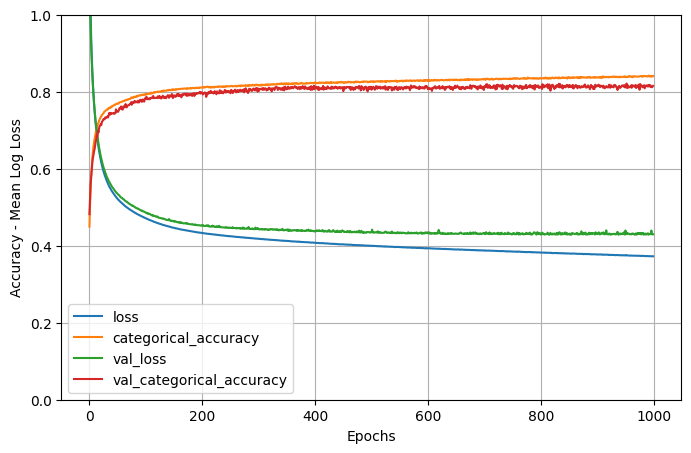
\includegraphics[scale=0.5]{tr-a1-e2.png}		
					\caption{Entrenamiento durante el Experimento 2 de la Arquitectura 1}	
					\label{tr-a1-e2}
				\end{center}
			\end{figure}
			En la figura \ref{tr-a1-e2} vemos que a partir del epoch 400 no hay una mejora en \textit{accuracy} para el conjunto de validaci\'on aunque s\'i para el conjunto de entrenamiento lo que nos indica que un n\'umero de \textit{epochs} tan elevado como el que hemos usado en este experimento con esta arquitectura y configuraci\'on conduce a un \textit{overfitting} del modelo, aunque por el momento no es excesivo como nos indica la \textit{variance}.
			
		\subsection{Experimento 3: Cambiamos a \textit{tanh} y reducimos \textit{epochs}}
		\label{s-a1-e3}
			Para este experimento decidimos reducir las \textit{epochs} ya que como hemos visto en el experimento anterior, no hay una mejora significativa en validaci\'on con m\'as epochs.\\
			Adem\'as de esto, cambiaremos la funci\'on de activaci\'on a \textit{tanh}. Hasta el momento hemos usado \textit{ReLU} pero no hay raz\'on para usarla para esta arquitectura porque resuelve el problema del \textit{vanishing gradient} que se da en arquitecturas profundas.\\
			La configuraci\'on que usamos para el experimento 3 es:
			\begin{table}[!h]
				\begin{center}
					\begin{tabular}{| c | c | c | c | c | c | c |}
						\textbf{Epochs} & \textbf{Learning rate} & \textbf{Batch size} & \textbf{Activation} & \textbf{Loss} & \textbf{Optimizer} & \textbf{Regularization} \\ \hline
						\textbf{400} & 0.1 & 512 & \textbf{tanh} & Categorical Crossentropy & SGD & None
					\end{tabular}
					\caption{Hiperpar\'ametros para el Experimento 3 de la Arquitectura 1}
					\label{tab:hip-a1-e3}
				\end{center}
			\end{table}
			
			Tras 5 entrenamientos obtenemos los siguientes resultados:
			\begin{table}[!h]
				\begin{center}
					\begin{tabular}{ c | c | c | c | c | c |}
						\ & \textbf{Train accuracy (\%)} & \textbf{Validation accuracy (\%)} & \textbf{Bias (\%)} & \textbf{Variance (\%)} & \textbf{Training time (s)} \\ \hline
						\textbf{Mean} & 79.58 & 78.3 & 15.41 & 1.28 & 72\\ \hline
						\textbf{Std} & 0.2 & 0.51 & 0.22 & 0.33 & 3.27 \\ \hline
					\end{tabular}
					\caption{Resultados del Experimento 3 de la Arquitectura 1}
					\label{tab:res-a1-e3}
				\end{center}
			\end{table}
			
			Con esta configuraci\'on el modelo ha vuelto a aumentar el \textit{bias} y obtenemos unos resultados pr\'acticamente id\'enticos al experimento uno con la funci\'on de activaci\'on \textit{ReLU} aunque con m\'as epochs. Parece que con la funci\'on \textit{tanh}, el modelo se queda atrapado en m\'inimos globales como podemos apreciar en la figura \ref{tr-a1-e3} y necesita m\'as epochs para escapar de ellos.\\
			
			\begin{figure}[!h]
				\begin{center}
					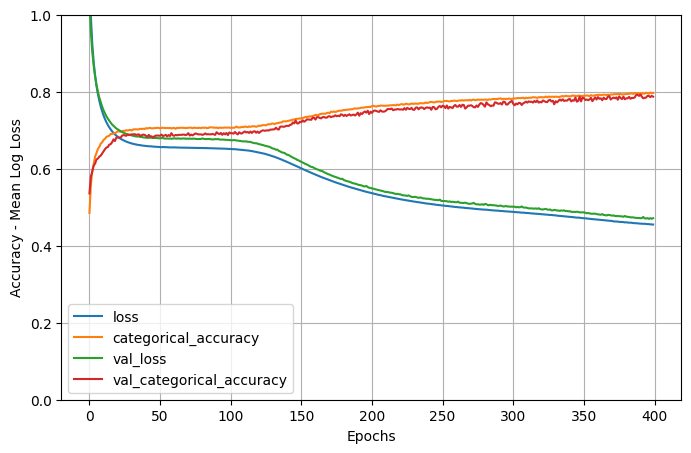
\includegraphics[scale=0.5]{tr-a1-e3.png}		
					\caption{Entrenamiento durante el Experimento 3 de la Arquitectura 1}	
					\label{tr-a1-e3}
				\end{center}
			\end{figure}
			
			Tambi\'en observamos que no ha habido overfitting hasta la epoch 400, al contrario de lo que hab\'iamos supuesto al inicio de este experimento.
			
		\subsection{Experimento 4: Aumentamos \textit{epochs}}
		\label{s-a1-e4}
			El objetivo de este experimento es comprobar cu\'antas \textit{epochs} podemos realizar antes de que el modelo comience a dirigirse hacia un \textit{overfitting} por lo que la configuraci\'on es la misma que en la ejecuci\'on anterior, excepto que volvemos a incrementar las epochs a 1000:
			\begin{table}[!h]
				\begin{center}
					\begin{tabular}{| c | c | c | c | c | c | c |}
						\textbf{Epochs} & \textbf{Learning rate} & \textbf{Batch size} & \textbf{Activation} & \textbf{Loss} & \textbf{Optimizer} & \textbf{Regularization} \\ \hline
						\textbf{1000} & 0.1 & 512 & tanh & Categorical Crossentropy & SGD & None
					\end{tabular}
					\caption{Hiperpar\'ametros para el Experimento 4 de la Arquitectura 1}
					\label{tab:hip-a1-e4}
				\end{center}
			\end{table}
			
			Tras 5 entrenamientos obtenemos los siguientes resultados:
			\begin{table}[!h]
				\begin{center}
					\begin{tabular}{ c | c | c | c | c | c |}
						\ & \textbf{Train accuracy (\%)} & \textbf{Validation accuracy (\%)} & \textbf{Bias (\%)} & \textbf{Variance (\%)} & \textbf{Training time (s)} \\ \hline
						\textbf{Mean} & 81.17 & 80.23 & 13.82 & 0.94 & 189\\ \hline
						\textbf{Std} & 0.14 & 0.62 & 0.14 & 0.53 & 2.3 \\ \hline
					\end{tabular}
					\caption{Resultados del Experimento 4 de la Arquitectura 1}
					\label{tab:res-a1-e4}
				\end{center}
			\end{table}
			
			\begin{figure}[!h]
				\begin{center}
					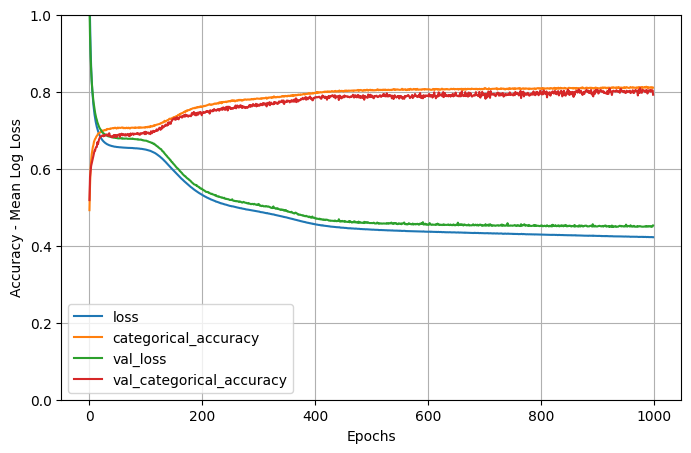
\includegraphics[scale=0.5]{tr-a1-e4.png}		
					\caption{Entrenamiento durante el Experimento 4 de la Arquitectura 1}	
					\label{tr-a1-e4}
				\end{center}
			\end{figure}
			
			Aunque hemos doblado las \textit{epochs} con respecto al experimento 3, la mejora ha sido de apenas un 2\% en \textit{accuracy}. Por otra parte, como se muestra en la figura \ref{tr-a1-e4}, el modelo no ha llegado al punto de \textit{overfitting} aun habiendo usado un n\'umero tan alto de epochs.\\
			Esto quiere decir que todav\'ia hay margen de mejora si seguimos entrenando con m\'as epochs aunque llevar\'ia mucho tiempo porque el aprendizaje es lento.\\
			
		\subsection{Experimento 5: Reducimos \textit{batch size}}
		\label{s-a1-e5}
			Como se necesitar\'ia aumentar exponencialmente el n\'umero de \textit{epochs} para conseguir una mejora en el \textit{accuracy}, decidimos reducir el \textit{batch size} y comprobar si de esta forma el modelo consigue mejores resultados.
			\begin{table}[!h]
				\begin{center}
					\begin{tabular}{| c | c | c | c | c | c | c |}
						\textbf{Epochs} & \textbf{Learning rate} & \textbf{Batch size} & \textbf{Activation} & \textbf{Loss} & \textbf{Optimizer} & \textbf{Regularization} \\ \hline
						1000 & 0.1 & \textbf{128} & tanh & Categorical Crossentropy & SGD & None
					\end{tabular}
					\caption{Hiperpar\'ametros para el Experimento 5 de la Arquitectura 1}
					\label{tab:hip-a1-e5}
				\end{center}
			\end{table}
			
			Tras 5 entrenamientos obtenemos los siguientes resultados:\\
			\begin{table}[!h]
				\begin{center}
					\begin{tabular}{ c | c | c | c | c | c |}
						\ & \textbf{Train accuracy (\%)} & \textbf{Validation accuracy (\%)} & \textbf{Bias (\%)} & \textbf{Variance (\%)} & \textbf{Training time (s)} \\ \hline
						\textbf{Mean} & 82.92 & 80.84 & 12.07 & 2.08 & 517.2\\ \hline
						\textbf{Std} & 0.19 & 0.29 & 0.19 & 0.28 & 25.61 \\ \hline
					\end{tabular}
					\caption{Resultados del Experimento 4 de la Arquitectura 1}
					\label{tab:res-a1-e5}
				\end{center}
			\end{table}
			Como vemos en la tabla \ref{tab:res-a1-e5} no conseguimos mejorar de forma significativa el \textit{accuracy}. Aumentar el \textit{batch size} ha incrementado exponencialmente el tiempo de entrenamiento por lo que no merece la pena reducir el \textit{batch size} en este caso. Lo que hemos conseguido reduciendo el \textit{batch size} ha sido que el modelo escape r\'apidamente del primer m\'inimo local con el que se topa como vemos en la figura \ref{tr-a1-e5} as\'i que concluimos que con esta t\'ecnica podemos obtener un resultado aceptable en menor tiempo.
			\begin{figure}[!h]
				\begin{center}
					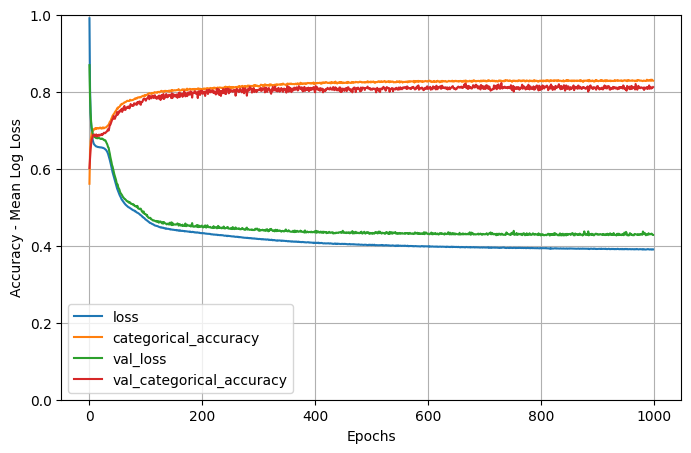
\includegraphics[scale=0.5]{tr-a1-e5.png}		
					\caption{Entrenamiento durante el Experimento 5 de la Arquitectura 1}	
					\label{tr-a1-e5}
				\end{center}
			\end{figure}
			
		\subsection{Conclusiones de la Arquitectura 1}
			\begin{itemize}
				\item \textit{ReLU} llega a un estado de \textit{overfitting} con menos \textit{epochs} que \textit{tanh}
				\item \textit{tanh} tiene un proceso de aprendizaje m\'as lento que \textit{ReLU}
				\item Reducir el \textit{batch size} implica llegar a un \'optimo de forma m\'as r\'apida con \textit{tanh}.
			\end{itemize}
			
	\section{Arquitectura 2: Deep Feed Forward Neural Network}
		Hemos visto que con la arquitectura anterior obtenemos un \textit{accuracy} m\'aximo de un 84\% a partir de donde el aprendizaje es lento y llegamos a un \textit{overfitting} con las t\'ecnicas utilizadas. Es por esto que decidimos usar una Deep Feed Forward Neural Network para intentar reducir el \textit{bias} del modelo.\\
		La arquitectura que utilizaremos para la nueva serie de experimento ser\'a:
		
		\begin{enumerate}
			\item Capa densa de 128 neuronas
			\item Capa densa de 64 neuronas
			\item Capa densa de 32 neuronas
		\end{enumerate}
		
		\subsection{Experimento 1: Comparaci\'on con arquitectura 1}
		\label{s-a2-e1}
			En este experimento utilizaremos la misma configuraci\'on que en el experimento anterior:
			\begin{table}[!h]
				\begin{center}
					\begin{tabular}{| c | c | c | c | c | c | c |}
						\textbf{Epochs} & \textbf{Learning rate} & \textbf{Batch size} & \textbf{Activation} & \textbf{Loss} & \textbf{Optimizer} & \textbf{Regularization} \\ \hline
						1000 & 0.1 & 128 & tanh & Categorical Crossentropy & SGD & None
					\end{tabular}
					\caption{Hiperpar\'ametros para el Experimento 1 de la Arquitectura 2}
					\label{tab:hip-a2-e1}
				\end{center}
			\end{table}
			
			Tras 5 entrenamientos obtenemos los siguientes resultados:
			
			\begin{table}[!h]
				\begin{center}
					\begin{tabular}{ c | c | c | c | c | c |}
						\ & \textbf{Train accuracy (\%)} & \textbf{Validation accuracy (\%)} & \textbf{Bias (\%)} & \textbf{Variance (\%)} & \textbf{Training time (s)} \\ \hline
						\textbf{Mean} & 99.89 & 74.97 & -4.89 & 24.91 & 578\\ \hline
						\textbf{Std} & 0.04 & 0.26 & 0.04 & 0.26 & 4.54 \\ \hline
					\end{tabular}
					\caption{Resultados del Experimento 1 de la Arquitectura 2}
					\label{tab:res-a2-e1}
				\end{center}
			\end{table}
			
			Hemos obtenido un modelo con un \textit{overfitting} muy alto, tan alto que ha cometido menos error que un humano y por eso el \textit{bias} es negativo. Podemos ver el \textit{overfitting} reflejado en el \textit{variance} de un 25\% de la tabla \ref{tab:res-a2-e1} y la evoluci\'on del \textit{validation categorical accuracy} en la figura \ref{tr-a2-e1} que empeora a lo largo del entrenamiento.
			
			\begin{figure}[!h]
				\begin{center}
					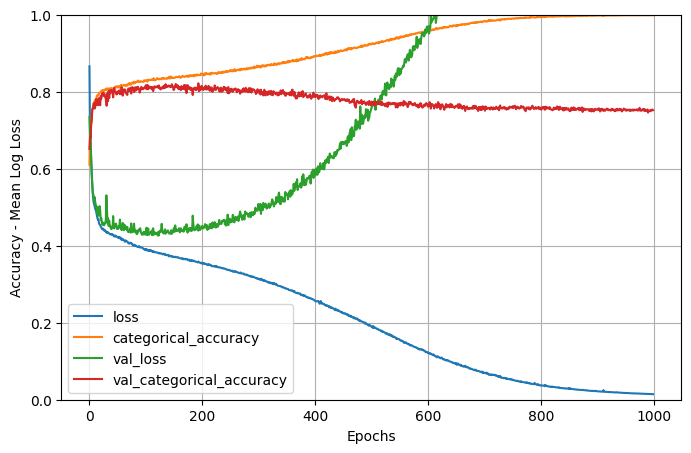
\includegraphics[scale=0.5]{tr-a2-e1.png}		
					\caption{Entrenamiento durante el Experimento 1 de la Arquitectura 2}	
					\label{tr-a2-e1}
				\end{center}
			\end{figure}
			
			\newpage
			
			
		\subsection{Experimento 2: Reducimos \textit{epochs} y utilizamos regularizaci\'on}
		\label{s-a2-e2}
			Una de las t\'ecnicas que podemos utilizar para reducir el \textit{variance} es usar regularizaci\'on para controlar que los pesos de las neuronas no se hagan demasiado grande. Adem\'as para ahorrar algo de tiempo tambi\'en reduciremos las epochs. La configuraci\'on para este experimento queda reflejada en la tabla \ref{tab:hip-a2-e2}.
			\begin{table}[!h]
				\begin{center}
					\begin{tabular}{| c | c | c | c | c | c | c |}
						\textbf{Epochs} & \textbf{Learning rate} & \textbf{Batch size} & \textbf{Activation} & \textbf{Loss} & \textbf{Optimizer} & \textbf{Regularization} \\ \hline
						\textbf{400} & 0.1 & 128 & tanh & Categorical Crossentropy & SGD & \textbf{l2 0.001}
					\end{tabular}
					\caption{Hiperpar\'ametros para el Experimento 2 de la Arquitectura 2}
					\label{tab:hip-a2-e2}
				\end{center}
			\end{table}
			
			Tras 5 entrenamientos obtenemos los siguientes resultados:
			
			\begin{table}[!h]
				\begin{center}
					\begin{tabular}{ c | c | c | c | c | c |}
						\ & \textbf{Train accuracy (\%)} & \textbf{Validation accuracy (\%)} & \textbf{Bias (\%)} & \textbf{Variance (\%)} & \textbf{Training time (s)} \\ \hline
						\textbf{Mean} & 81.19 & 79.91 & 13.8 & 1.28 & 249\\ \hline
						\textbf{Std} & 0.2 & 0.95 & 0.2 & 0.92 & 3.29 \\ \hline
					\end{tabular}
					\caption{Resultados del Experimento 2 de la Arquitectura 2}
					\label{tab:res-a2-e2}
				\end{center}
			\end{table}
			
			Como se observa en la tabla \ref{tab:res-a2-e2}, hemos conseguido reducir el \textit{variance} un 24\% simplemente usando regularizaci\'on, ahora bien, en cuanto a \textit{accuracy} seguimos sin conseguir una mejora significativa.
			
			\begin{figure}[!h]
				\begin{center}
					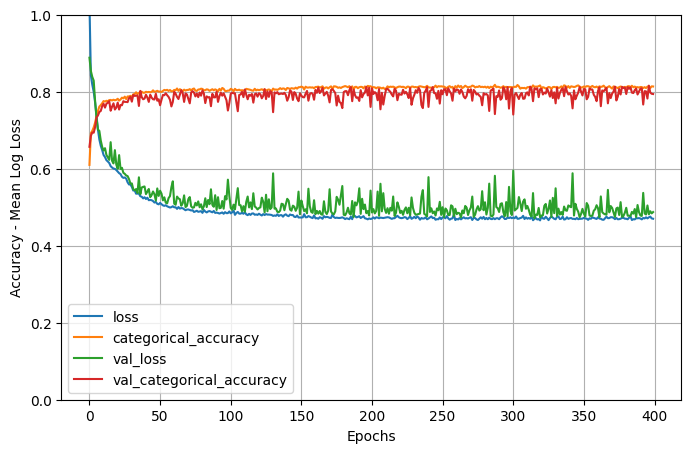
\includegraphics[scale=0.5]{tr-a2-e2.png}		
					\caption{Entrenamiento durante el Experimento 2 de la Arquitectura 2}	
					\label{tr-a2-e2}
				\end{center}
			\end{figure}
			
			En la figura \ref{tr-a2-e2} se aprecia ruido en las m\'etricas del conjunto de validaci\'on, esto es una consecuencia de la regularizaci\'on, sin ella ese ruido se descontrolar\'ia y llegar\'iamos al \textit{overfitting} como en el experimento anterior.
			
			
		\subsection{Experimento 3: Cambiamos el optimizador}
		\label{s-a2-e3}
			En este experimento vamos a comprobar si con un optimizador distinto podemos obtener mejor \textit{accuracy} sin llegar al \textit{overfitting}, para ello utilizaremos ADAM. La configuraci\'on es la siguiente:
			
			\begin{table}[!h]
				\begin{center}
					\begin{tabular}{| c | c | c | c | c | c | c |}
						\textbf{Epochs} & \textbf{Learning rate} & \textbf{Batch size} & \textbf{Activation} & \textbf{Loss} & \textbf{Optimizer} & \textbf{Regularization} \\ \hline
						400 & 0.1 & 128 & tanh & Categorical Crossentropy & \textbf{ADAM} & l2 0.001
					\end{tabular}
					\caption{Hiperpar\'ametros para el Experimento 3 de la Arquitectura 2}
					\label{tab:hip-a2-e3}
				\end{center}
			\end{table}
			
			\newpage
			Tras 5 entrenamientos obtenemos los siguientes resultados:
			
			\begin{table}[!h]
				\begin{center}
					\begin{tabular}{ c | c | c | c | c | c |}
						\ & \textbf{Train accuracy (\%)} & \textbf{Validation accuracy (\%)} & \textbf{Bias (\%)} & \textbf{Variance (\%)} & \textbf{Training time (s)} \\ \hline
						\textbf{Mean} & 25.34 & 26.25 & 69.65 & -0.91 & 266.8 \\ \hline
						\textbf{Std} & 0.29 & 2.61 & 0.29 & 2.44 & 4.81 \\ \hline
					\end{tabular}
					\caption{Resultados del Experimento 3 de la Arquitectura 2}
					\label{tab:res-a2-e3}
				\end{center}
			\end{table}
			
			Como vemos en la tabla resultados son los peores obtenidos hasta el momento y con mucha diferencia, apenas hemos conseguido un 25\% de \textit{accuracy}. Analizando la figura \ref{tr-a2-e3}, el modelo se queda estancado en un m\'inimo local muy temprano en el entrenamiento.
			\begin{figure}[!h]
				\begin{center}
					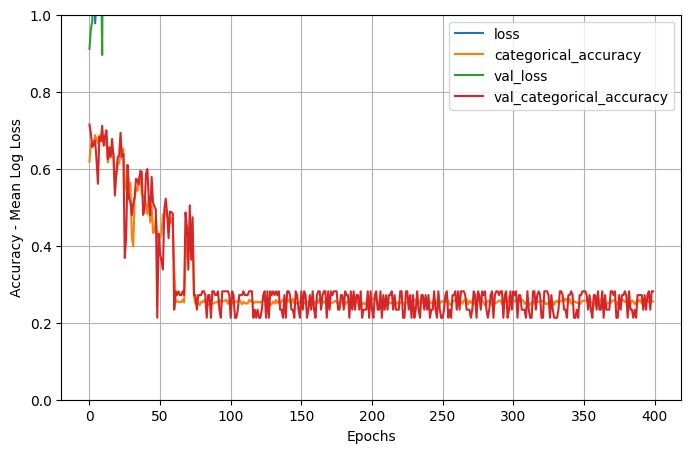
\includegraphics[scale=0.5]{tr-a2-e3.png}		
					\caption{Entrenamiento durante el Experimento 4 de la Arquitectura 2}	
					\label{tr-a2-e3}
				\end{center}
			\end{figure}
			
			Observando la matriz de confusi\'on confirmamos nuestra teor\'ia, clasifica todos los jugadores en la misma clase.
			\begin{figure}[!h]
				\begin{center}
					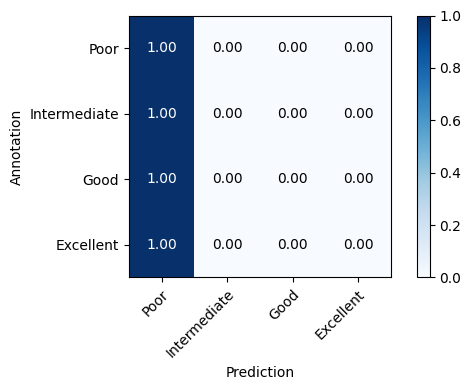
\includegraphics[scale=0.7]{cm-a2-e3.png}		
					\caption{Matriz de confusi\'on en el Experimento 3 de la Arquitectura 2}	
					\label{cm-a2-e3}
				\end{center}
			\end{figure}
			
			Esto puede deberse a que no estamos usando correctamente el optimizador ADAM.
			
			
		\subsection{Experimento 4: Ajustamos el optimizador ADAM}
		\label{s-a2-e4}
			Consultando el art\'iculo en el que se present\'o ADAM (\textit{Adam: A Method for Stochastic Optimization}, (2015), D. Kingma y J. Ba), vemos que este optimizador es una combinaci\'on entre AdaGrad y RMSProp y que tiene unos par\'ametros que controlan el ratio de decrecimiento de los momentos (beta1=0.9 y beta2=0.999) que no hemos definido en el experimento anterior. Adem\'as de esto, los autores sugieren usar un \textit{learning rate} m\'as bajo del que estamos usando.\\
			
			La configuraci\'on queda as\'i:
			\begin{table}[!h]
				\begin{center}
					\begin{tabular}{| c | c | c | c | c | c | c |}
						\textbf{Epochs} & \textbf{Learning rate} & \textbf{Batch size} & \textbf{Activation} & \textbf{Loss} & \textbf{Optimizer} & \textbf{Regularization} \\ \hline
						400 & \textbf{0.001} & 128 & tanh & Categorical Crossentropy & ADAM & l2 0.001
					\end{tabular}
					\caption{Hiperpar\'ametros para el Experimento 4 de la Arquitectura 2}
					\label{tab:hip-a2-e4}
				\end{center}
			\end{table}
			
			Tras 5 entrenamientos obtenemos los siguientes resultados:
			
			\begin{table}[!h]
				\begin{center}
					\begin{tabular}{ c | c | c | c | c | c |}
						\ & \textbf{Train accuracy (\%)} & \textbf{Validation accuracy (\%)} & \textbf{Bias (\%)} & \textbf{Variance (\%)} & \textbf{Training time (s)} \\ \hline
						\textbf{Mean} & 81.97 & 80.48 & 13.02 & 1.49 & 250.2 \\ \hline
						\textbf{Std} & 0.15 & 0.15 & 0.15 & 0.19 & 19.35 \\ \hline
					\end{tabular}
					\caption{Resultados del Experimento 4 de la Arquitectura 2}
					\label{tab:res-a2-e4}
				\end{center}
			\end{table}
			
			Al haber configurado correctamente el optimizador volvemos a conseguir un \textit{accuracy} similar al que hemos estado obteniendo. Observando la figira \ref{tr-a2-e4} vemos qe podr\'iamos seguir entrenando el modelo por m\'as \textit{epochs} antes de llegar al \textit{overfitting}. Aun con todo esto, no hemos obtenido mejores resultados que con el optimizador \textit{SGD}.
			\begin{figure}[!h]
				\begin{center}
					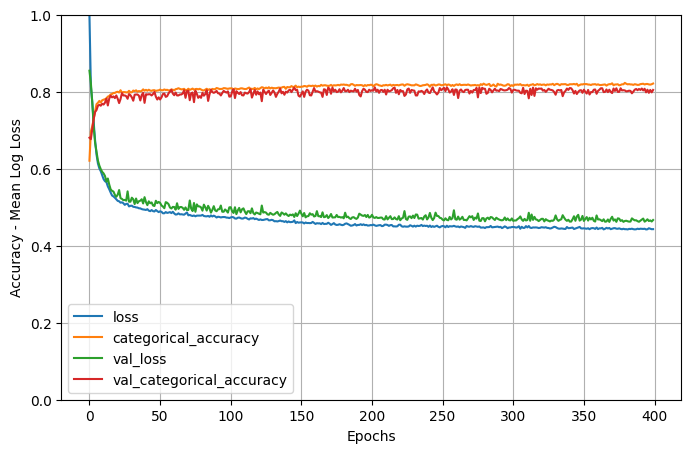
\includegraphics[scale=0.5]{tr-a2-e4.png}		
					\caption{Entrenamiento durante el Experimento 4 de la Arquitectura 2}	
					\label{tr-a2-e4}
				\end{center}
			\end{figure}
			
			Analizando la matriz de confusi\'on en la figura \ref{cm-a2-e4} vemos que ahora hemos solucionado el problema del modelo anterior que clasificaba todos los jugadores en la misma clase
			\begin{figure}[!h]
				\begin{center}
					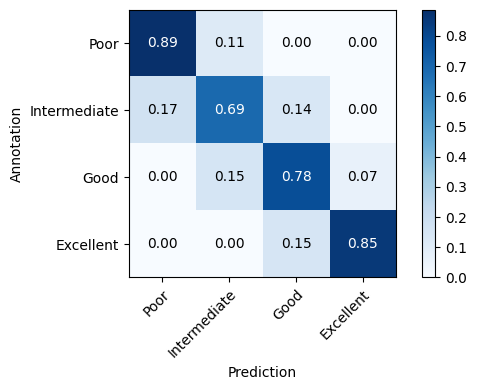
\includegraphics[scale=0.7]{cm-a2-e4.png}		
					\caption{Matriz de confusi\'on en el Experimento 4 de la Arquitectura 2}	
					\label{cm-a2-e4}
				\end{center}
			\end{figure}
		\newpage
		\subsection{Experimento 5: Reducimos \textit{batch-size}}
		\label{s-a2-e5}
			Decidimos reducir el \textit{batch size} para intentar reducir el \textit{bias} como en el experimento \ref{s-a1-e5}. La configuraci\'on para este experimento es:
			\begin{table}[!h]
				\begin{tabular}{| c | c | c | c | c | c | c |}
					\textbf{Epochs} & \textbf{Learning rate} & \textbf{Batch size} & \textbf{Activation} & \textbf{Loss} & \textbf{Optimizer} & \textbf{Regularization} \\ \hline
					400 & 0.001 & \textbf{64} & tanh & Categorical Crossentropy & ADAM & l2 0.001
				\end{tabular}
				\caption{Hiperpar\'ametros para el Experimento 5 de la Arquitectura 2}
				\label{tab:hip-a2-e5}
			\end{table}
			
			Tras 5 entrenamientos obtenemos los siguientes resultados:
			
			\begin{table}[!h]
				\begin{center}
					\begin{tabular}{ c | c | c | c | c | c |}
						\ & \textbf{Train accuracy (\%)} & \textbf{Validation accuracy (\%)} & \textbf{Bias (\%)} & \textbf{Variance (\%)} & \textbf{Training time (s)} \\ \hline
						\textbf{Mean} & 81.87 & 80.03 & 13.12 & 1.83 & 506.4 \\ \hline
						\textbf{Std} & 0.22 & 0.77 & 0.22 & 0.89 & 38.48 \\ \hline
					\end{tabular}
					\caption{Resultados del Experimento 5 de la Arquitectura 2}
					\label{tab:res-a2-e5}
				\end{center}
			\end{table}
			
			\begin{figure}[!h]
				\begin{center}
					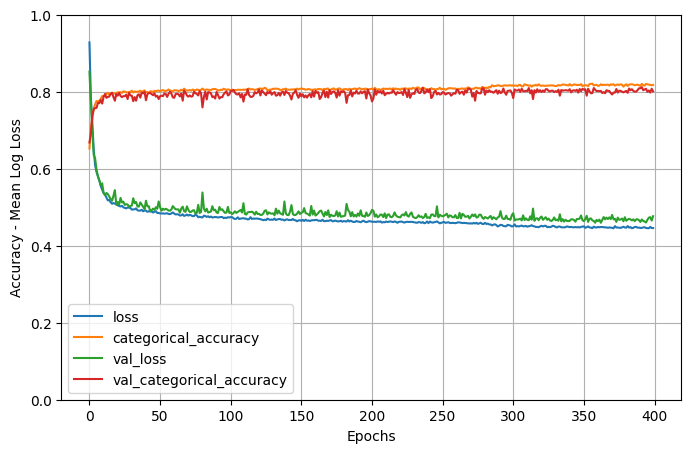
\includegraphics[scale=0.5]{tr-a2-e5.png}		
					\caption{Entrenamiento durante el Experimento 5 de la Arquitectura 2}	
					\label{tr-a2-e5}
				\end{center}
			\end{figure}
			
			\newpage
			No hemos obtenido mejora, este cambio no merece la pena porque aumenta mucho el tiempo de entrenamiento. Como vemos en la figura \ref{tr-a2-e5}, parece que el modelo deja de aprender, quiz\'as por el problema del \textit{vanishing gradient} que intentaremos resolver con la siguiente arquitectura.
		
		\subsection{Conclusiones de la Arquitectura 2}
			A lo largo de estos experimentos hemos concluido que:
			\begin{itemize}
				\item La regularizaci\'on evita el \textit{overfitting}.
				\item El optimizador ADAM necesita un \textit{learning rate} bajo.
				\item El optimizador ADAM no ha proporcionado mejoras significativas con respecto al SGD para esta arquitectura.
			\end{itemize}
			
	\section{Arquitectura 3: Batch normalization}
		Despu\'es de no conseguir reducir el \textit{bias} de nuestro modelo con m\'as capas ocultas suponemos que estamos ante un problema de \textit{vanishing gradient}, una de las soluciones que existe es utilizar capas de \textit{batch normalization} para estandarizar los pesos de las neuronas. La arquitectura que utilizaremos durante los siguientes experimentos es:
		\begin{enumerate}
			\item Capa densa de 128 neuronas
			\item Capa de \textit{Batch Normalization} antes de la activaci\'on.
			\item Capa densa de 64 neuronas
			\item Capa de \textit{Batch Normalization} antes de la activaci\'on.
			\item Capa densa de 32 neuronas
			\item Capa de \textit{Batch Normalization} antes de la activaci\'on.
		\end{enumerate}
		
		\subsection{Experimento 1: Probamos la configuraci\'on del experimento \ref{s-a2-e5}}
			Para comprobar como afecta la introducci\'on del \textit{batch normalization}, utilizamos la configuraci\'on del \'ultimo experimento realizado.
			
			\begin{table}[!h]
				\begin{tabular}{| c | c | c | c | c | c | c |}
					\textbf{Epochs} & \textbf{Learning rate} & \textbf{Batch size} & \textbf{Activation} & \textbf{Loss} & \textbf{Optimizer} & \textbf{Regularization} \\ \hline
					400 & 0.001 & 64 & tanh & Categorical Crossentropy & ADAM & l2 0.001
				\end{tabular}
				\caption{Hiperpar\'ametros para el Experimento 1 de la Arquitectura 3}
				\label{tab:hip-a3-e1}
			\end{table}
			
			Tras 5 entrenamientos obtenemos los siguientes resultados:
			
			\begin{table}[!h]
				\begin{center}
					\begin{tabular}{ c | c | c | c | c | c |}
						\ & \textbf{Train accuracy (\%)} & \textbf{Validation accuracy (\%)} & \textbf{Bias (\%)} & \textbf{Variance (\%)} & \textbf{Training time (s)} \\ \hline
						\textbf{Mean} & 89.23 & 76.23 & 5.76 & 15.59 & 950.4 \\ \hline
						\textbf{Std} & 0.46 & 1.54 & 0.46 & 1.75 & 55.11 \\ \hline
					\end{tabular}
					\caption{Resultados del Experimento 1 de la Arquitectura 3}
					\label{tab:res-a3-e1}
				\end{center}
			\end{table}
			La tabla \ref{tab:res-a3-e1} nos muestra que con \textit{batch normalization} hemos obtenido una buena \textit{accuracy} en el conjunto de entrenamiento pero a cambio de obtener un modelo con \textit{overfitting} como nos indica el \textit{variance} de 15\%. Tambi\'en ha sido la ejecuci\'on m\'as larga dado el tama\~no del batch y que hemos usado \textit{batch normalization} que ralentiza el proceso de entrenamiento.
			\newpage
			 
			\begin{figure}[!h]
				\begin{center}
					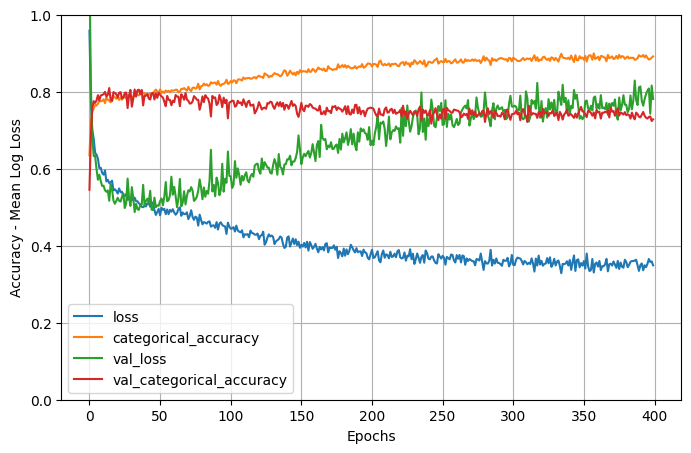
\includegraphics[scale=0.5]{tr-a3-e1.png}		
					\caption{Entrenamiento durante el Experimento 1 de la Arquitectura 3}	
					\label{tr-a3-e1}
				\end{center}
			\end{figure}
			
			En la figura \ref{tr-a3-e1} vemos como el modelo llega al punto de \textit{overfit} alrededor de la \textit{epoch} 50 donde el \textit{accuracy} de validaci\'on se separa del de entrenamiento.
			
			\subsection{Experimento 2: Aumentamos \textit{batch size}}
				A\'un no hemos conseguido mejorar el \textit{accuracy} en el conjunto de validaci\'on, pero en este experimento vamos a intentar retrasar el \textit{overfitting} del modelo a la vez que el tiempo de entrenamiento aumentando el \textit{batch size}
\end{document}
